\documentclass[12pt]{article}
\usepackage[a4paper]{geometry}
%\userpackage[top=1 in, bottom=1.25 in, left=1.1 in, rigth=1.1 in] {geometry}
%\usepackage[paperwidth=17cm, paperheight=22.5cm, bottom=2.5cm, right=2.5cm]{geometry}
\usepackage[utf8]{inputenc}
%\usepackage[a4paper, top=2.5cm, bottom=2.5cm, left=2.2cm, right=2.2cm]
%{geometry}
%\usepackage[myheadings]{fullpage}
\usepackage{fancyhdr}
\usepackage{lastpage}
%\usepackage{float}
\usepackage{graphicx, wrapfig, subcaption, setspace, booktabs}
\usepackage{graphicx}
\usepackage[T1]{fontenc}
\usepackage[font=small, labelfont=bf]{caption}
%\usepackage{fourier}
\usepackage[protrusion=true, expansion=true]{microtype}
\usepackage[english]{babel}
\usepackage{sectsty}
\usepackage{url, lipsum}
\usepackage[T1]{fontenc}
\usepackage{icomma}
\usepackage{siunitx}
\usepackage{ragged2e}
\usepackage{amsmath}
\usepackage{comment}
\usepackage{enumerate}
%\usepackage{changepage}
\usepackage{anysize}




\newcommand{\HRule}[1]{\rule{\linewidth}{#1}}
\onehalfspacing
\setcounter{tocdepth}{5}
\setcounter{secnumdepth}{5}

%-------------------------------------------------------------------------------
% HEADER & FOOTER
%-------------------------------------------------------------------------------


\begin{comment}
-Udledninger
$$
\begin{aligned}


\end{aligned}
$$

-Opgavetekst
\begin{figure}[H]
\includegraphics[width=0.5\textwidth]{"path"}
\end{figure} 


-Opgave billede med tekst
\begin{figure}[H]
\caption{"Billedtekst"}
\includegraphics[width=0.5\textwidth]{"path"}
\end{figure} 

-Værdier
$\\

$


\end{comment}
\begin{document}

\begin{titlepage}

\title{ \normalsize 
		%\begin{figure}
        \begin{center}
        
\includegraphics[height=6cm]{Logo.jpg}
        \end{center}
       % \end{figure}
        \LARGE \textsc{\textbf{Universidad De Sonora}} \\ \bigskip
		\Large División de Ciencias Exactas y Naturales \\
        Licenciatura En Física \\ \bigskip
        \bigskip
        Física Computacional I
		\\ [0.1cm]  
		\HRule{2pt} \\
		\Large \textbf{{Reporte de Actividad 4}} \\
        \textit{\textbf{"Introducción a la Programación de los Intérpretes de Comandos"}}
		\HRule{2pt} \\
		\normalsize \vspace*{0.001\baselineskip}}
        
\date{\bigskip \Large Hermosillo, Sonora  \hspace*{\fill}  Febrero 21 de 2018}

        
\author{
		\Large\textbf{ César Omar Ramírez Álvarez} \\ \bigskip
        \\ \bigskip
       \Large Profr. Carlos Lizárraga Celaya}
       \end{titlepage}
       \maketitle
       

\newpage
\pagestyle{plain}
\section*{Introducción}
Los sistemas operativos UNIX y otros sistemas derivados, como lo es Linux y macOS, se apoyan con un intérprete de comandos (Shell), quien juega el papel de intermediario entre el usuario y el sistema operativo. Un \textit{Shell} es una interfaz de usuario para acceder a los servicios de un sistema operativo.\\

En general, las shells del sistema operativo utilizan una interfaz de línea de comandos (CLI) o una interfaz gráfica de usuario (GUI), dependiendo del rol de la computadora y de la operación particular. Se denomina shell porque es la capa más externa alrededor del núcleo del sistema operativo.\\

En la práctica de la semana se realizaron distintas acciones con el inteprete de comandos Shell. Fue utilizado para descarga de datos en conjunto, organización y filtración de los mismos, así como para crear archivos. \\

Durante el desarrollo del presente reporte se mostrará de forma general los aspectos prácticos necesarios para la realización de la actividad con los diferentes interpretes de comandos, como lo fueron el uso del cat, chmod, echo, grep, etc. Incluyendo una descripción teórica a grandes rasgos de éstos. Por último a menara de síntesis se presenta un tutorial de Shell mostrando varios ejemplos rescatados de una página web recomendada. 

\section*{Práctica y Resultados}
Como una primera acción fue descargar y guardar en la carpeta Actividad 4 el archivo proporcionado por el profesor. El archivo continene un script llamado "script.sh" que permite descargar de manera automática los registros de todos los días del año de una estación seleccionada de los sondeos atmosféricos. \\

Entrando en contexto, en la práctica anterior se trabajó con registros de solo dos meses, los cuales fueron descargados de manera individual. En esta ocasión, la descarga será automática y en conjunto por lo que se editó el script descargado colocando el número de la estación deseada. La estación con la que he trabajado es \textit{Camborne Observations}.\\

Los registros de sondeos atmosféricos son tomados de la Universidad de Wyoming en la página web siguiente (http://weather.uwyo.edu/upperair/sounding.html).\\

A continuación se presenta el script utilizado:
\begin{center}
	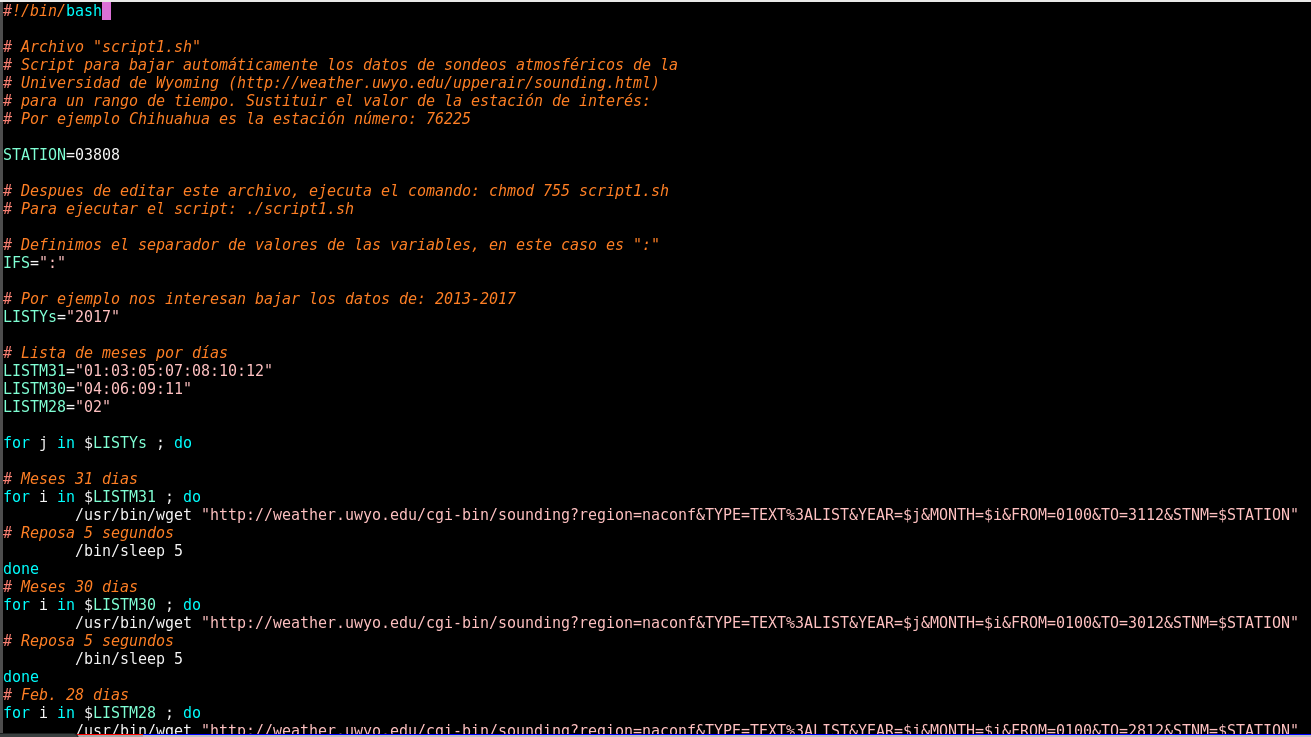
\includegraphics[height=9cm]{scriptdescarga.png}
\end{center}

La finalidad del script.sh, era descargar automáticamente los registros de todo un año de los sondeos meteorológicos de Camborne Observations , la cuál, es la estación con la que he trabajado. En el contenido del script es visible como estan declaradas las cosas, pues son variables tanto la estación como los meses (aclarando que para estos se definen la cantidad de días correspondientes, así evitamos datos basura) y se realizan ciclos "DO" dependiendo de los días que contiene cada mes, dejando descanso de 5 segundos entre mes y mes. Descarga los datos usando un comando llamada wget.\\

Éste script descargado con cuenta con el permiso para ser ejecutado, desde nuestra terminal con el comando "ls -alg" hacemos que se muestren los archivos y el tipo de permiso que éstos cuentan, notamos que nuestro archivo tiene los permisos: -rw-r–r–, que significa que es solamente de lectura para el dueño, posteriormente con el comando "chmod" cambiamos los permisos del archivo. Esto se hace posible mediante un cambio a notación en base 8, donde para este caso se utiliza 755. Usamos de nuevo el comando "ls -alg" y verificamos que ya es ejecutable.
\begin{center}
	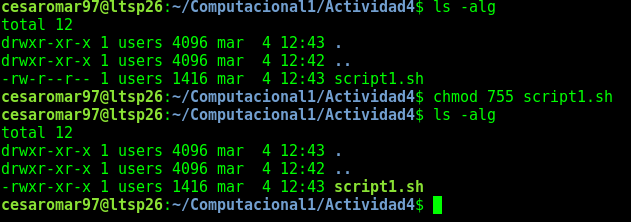
\includegraphics[height=4cm]{permiso.png}
\end{center}
Siendo ejecutable el script podemos correrlo y observamos el progreso de descarga de cada uno de los 12 archivos correspondientes.
\begin{center}
	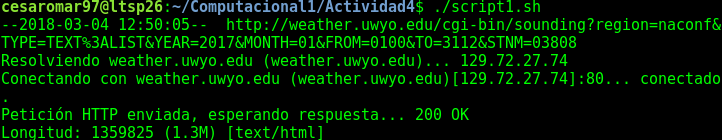
\includegraphics[height=3cm]{descargando.png}
\end{center}
\begin{center}
	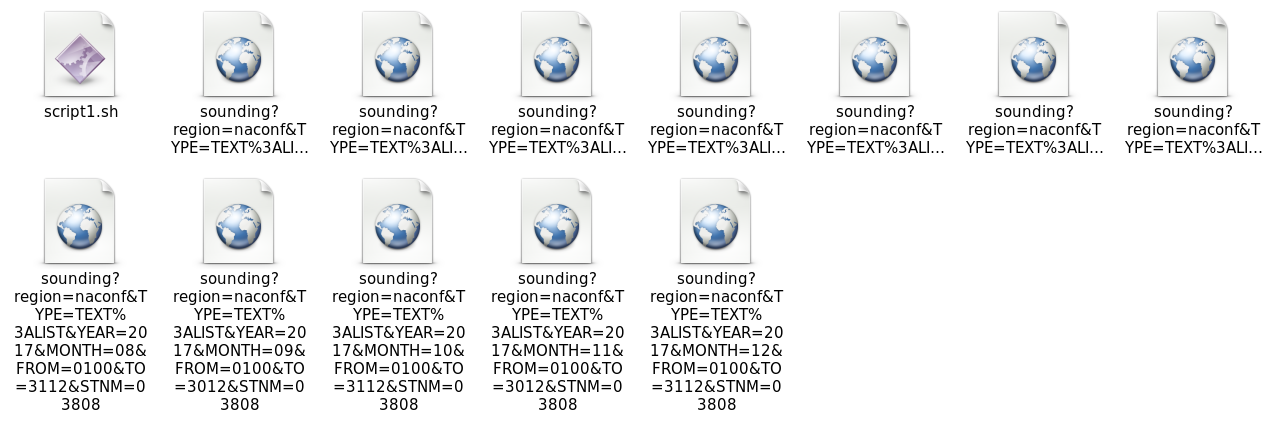
\includegraphics[height=4cm]{listo.png}
\end{center}
\begin{center}
	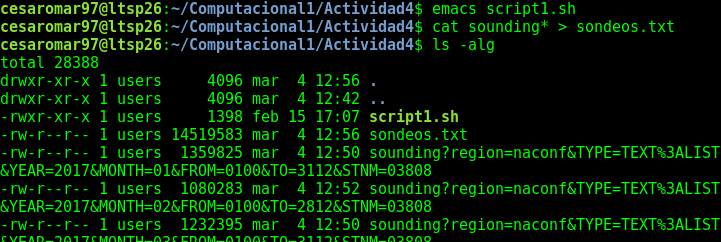
\includegraphics[height=4cm]{contenido.png}
\end{center}
Continuando, para el caso de lectura y revisión de los datos, hicimos uso de dos comandos muy parecidos en cierta forma, estos comandos son "less" y "cat". Ambos muestran en la terminal todos los datos de un archivo sin la posibilidad de editarlo, solo examinar datos se prdria decir. La única diferencia entre estos dos comandos es que el cursor cuando aplicamos less aparece al inicio del archivo y cuando aplicamos cat lo manda al final. 
\begin{center}
	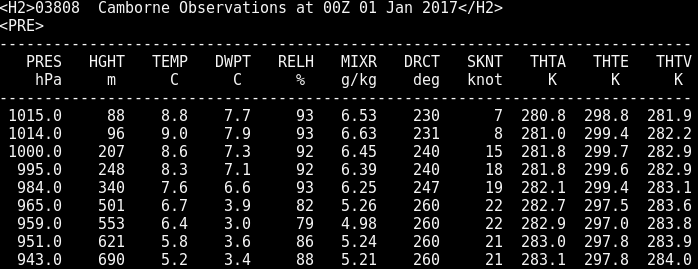
\includegraphics[height=4cm]{datos.png}
\end{center}
Otro comando utilizado es el "grep" que nos permite tomar cierta información en específico de un archivo renglón por renglón (si la hay). La manera de hacerlo es primeramente indicando el comando, la palabra o frase a buscar y el archivo de donde quieres que se busque.
\begin{center}
	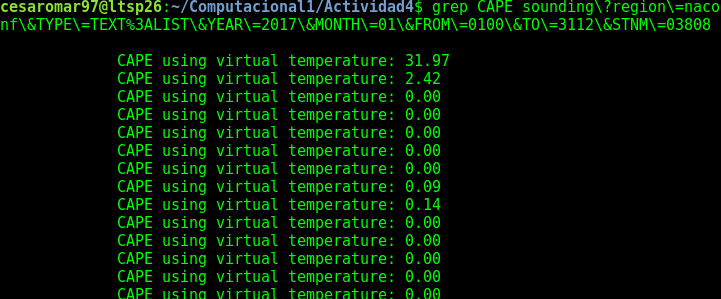
\includegraphics[height=4cm]{buscando.png}
\end{center}
Ahora bien, teniendo los archivos decargados verificamos a qué tipo pertenecen con el comando "file" esta vez agregando sounding* (por el hecho de que sounding* es el inicio de todos los archivos descargados y queremos saber el tipo de todos ellos) y notamos que son archivos de texto ASCII.
\begin{center}
	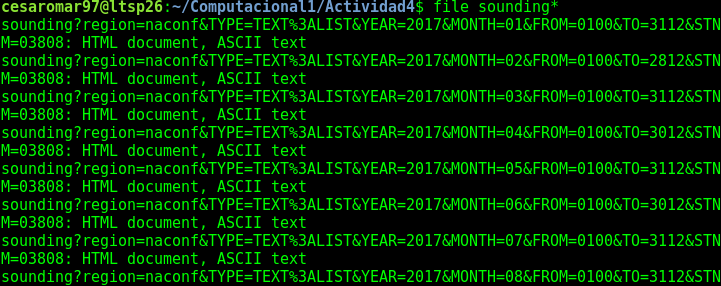
\includegraphics[height=4cm]{file.png}
\end{center}
Nos piden juntar todos los archivos en uno solo, por lo que  usaremos el comando cat pero agregandole un redirector ">" para indicar que todos estos archivos irán a un archivo .txt. Con esto ahora tenemos un archivo "sondeos.txt". A continuación, hicimos uso de grep, para filtrar los renglones de información que se quiere conservar (la deseada). Esto crea un archivo llamado df2017.csv, éstas ultimas dos acciones realizadas pueden ser automatizadas mediante el uso de
un scripts. En la actividad nos piden crear un script que contenga estas dos indicaciones con ayuda de él estas acciones podrán hacerse rápidamente sin la necesidad de hacerlo manualmente. Se crea el script con el editor de textos emacs colocando los comandos neceasiors (los anteriores), con un cambio solamente en el archivo de destino, llamandolo df2017\_2.csv. \\
\begin{verbatim}
egrep -v 'PRES|hPa' sondeos.txt | egrep '03808|Showalter|...|Precip' > df2017.csv
\end{verbatim}
\begin{center}
	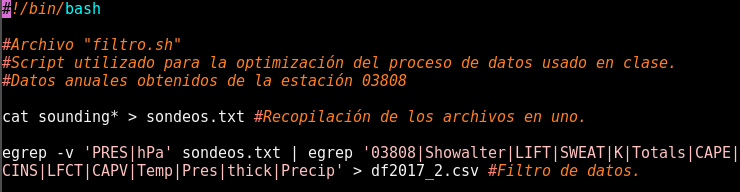
\includegraphics[height=4cm]{filtro.png}
\end{center}
\begin{center}
	
\includegraphics[height=2cm]{archis.png}
\end{center}
\begin{center}
	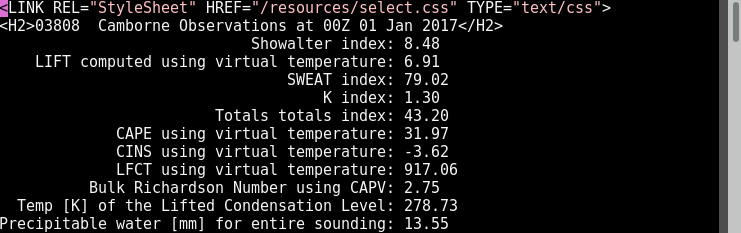
\includegraphics[height=4cm]{df2.png}
\end{center}
Teniendo estos dos archivos, como no cambio nada en su contenido, solo la forma de hacerlo (manual y automático) no debe existir ninguna diferencia. Para comprobar eso se hace uso del comando "diff", si existe tal diferencia la muestra en la terminal y si no, no muestra nada.
\begin{center}
	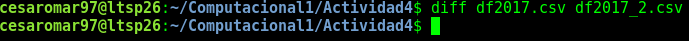
\includegraphics[height=0.8cm]{diff.png}
\end{center}

\subsection*{Breve Descripción de Comandos Utilizados}
\begin{itemize}
\item \textit{\textbf{cat: }}	Muestra el contenido de archivos y concatena archivos.
\item \textbf{\textit{ls: }} Lista archivos y directorios. Al agregar \textit{"-alg"} muestra los permisos de los archivos y directorios.
\item \textbf{\textit{chmod:}} Cambia los permisos de un archivo o carpetas.
\item \textbf{\textit{diff:}} Busca y muestra diferencias entre archivos.
\item \textit{\textbf{echo:}} Imprime una línea de texto, variables, o contenido a un archivo.
\item \textbf{\textit{file:}} Determina el tipo de archivo.
\item \textit{\textbf{grep:}} Busca patrones de cadenas dentro de archivos.
\item \textbf{\textit{less:}} Muestra el contenido de un archivo, permite búsquedas y movimento hacía atrás y adelante.
\item \textit{\textbf{wget:}} Descargador de archivos desde Internet, no interactivo.
\item \textbf{\textit{wc:}} Cuenta palabras, líneas, caracteres de un archivo o listado.
\item \textit{\textbf{redirectores:}} "|" separa datos, ">" envia información (datos o texto) a un archivo.
\end{itemize}

\section*{Síntesis \textbf{\textit{"Shell Script Tutorial"}}}
\subsection*{Introducción}

Este tutorial está escrito para ayudar a las personas a comprender algunos de los conceptos básicos de la programación de scripts de shell (también conocido como shell scripting ), y con suerte para presentar algunas de las posibilidades de la programación simple pero potente disponible bajo el shell Bourne. Está dirigido a la audiencia con conocimientos básicos en programación en Unix/ Linux Shell, es preferiblemente necesario conocer algunos comandos más comunes (\textit{ls, echo, cp, etc.}).

\subsection*{Filosofía}
La programación de script de Shell tiene una mala impresión entre algunos administradores de sistemas de Unix. Esto debido a la velocidad a la que se ejecutará un programa interpretado en comparación con un programa C y a la existencia de muchos scripts de shell de mala calidad. Es de suma importancia conocer los comandos para realizar un buen script y mantenerlo limpio.

\subsection*{Un Primer Script}
Para nuestro primer script de shell, solo escribiremos un script que diga "Hello World". El código es:
\begin{verbatim}
#!/bin/sh
# Este es un comentario!
echo Hola Mundo        # Este también es un comentario!
\end{verbatim}
La primera línea le dice a Unix que el archivo debe ser ejecutado por / bin / sh. La segunda línea comienza con un símbolo especial: \#. Esto marca la línea como un comentario, y el caparazón lo ignora por completo. La única excepción es cuando la primera línea del archivo comienza con \#!- como lo hace la nuestra.
Por ultimo el tercer renglón contiene el comando echo, el cual imprime en  pantalla lo que se escribe después del punto.
Podemos observar que echo automáticamente puso un espacio entre las palabras, pero si colocamos mas espacios shell lo interpretará como solamente uno, para poder realizar cambios de este estilo, debemos de colocar el texto entre comillas:
\begin{verbatim}
#!/bin/sh
# Este es un comentario!
echo "Hola      Mundo"       # Este también es un comentario!
\end{verbatim}
\begin{center}
	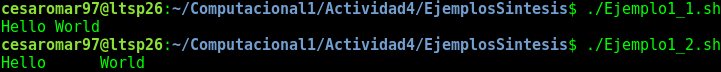
\includegraphics[height=1.5cm]{hello.png}
\end{center}
\subsection*{Variables I}
En casi todos los lenguajes de programación existe el concepto de variables, un nombre simbólico a un trozo de memoria al cual podemos asignarle un valor, leer y manipular su contenido. Para asignar variables se debe de igualar el nombre de la variable a lo que se desea almacenar, pero sin espacios.
\begin{verbatim}
#!/bin/sh
MY_MESSAGE="Hello World"
echo $MY_MESSAGE
\end{verbatim}
A shell no le importa el tipo de variable, pueden contener caracteres, enteros, reales, lo que se necesite. Pero si sabe diferenciar entre ellos. Por lo que ástas se debe mantener del mismo tipo y no intentar mezclar números con letras. Inclusive se puede utilizar variables junto con el comando read para leer un dato insertado de entrada y depositarlo en la variable.
\begin{verbatim}
#!/bin/sh
echo What is your name?
read MY_NAME
echo "Hello $MY_NAME - hope you’re well."
\end{verbatim}
Cabe resaltar que las variables se reinician cada vez que ejecutamos el script. Además si queremos juntar nuestra variable con otro dato, se hace entre corchetes curvos (llaves) para anunciar cuando inicia y acaba la variable, para que no lo considere todo. 
\begin{verbatim}
#!/bin/sh
echo "What is your name?"
read USER_NAME
echo "Hello $USER_NAME"
echo "I will create you a file called ${USER_NAME}_file"
touch "${USER_NAME}_file"
\end{verbatim}

\subsection*{Wildcards (Comodines)}
Son solamente comandos para utilizar en la terminal con la finalidad de facilitar el movimiento y edición de archivos de distintas sintaxis. Como un ejemplo, si queremos copiar los archivos de la carpeta "a" a la carpeta "b", es necasario usar el siguiente código:
\begin{verbatim}
$ cp /tmp/a/* /tmp/b/
$ cp /tmp/a/*.txt /tmp/b/
$ cp /tmp/a/*.html /tmp/b/
\end{verbatim}
Por lo general, se usan los wilcards para movimiento de archivos, y nos es tan común su uso en los scritps.

\subsection*{Caracteres de Escape}
Algunos caracteres tienen significado en shell, como ejemplo tenemos a las dobles comillas que afectan en como se tratan los espacios en el comando echo. Pero si deseamos utilizar las comillas como texto es necasario hcaer uso de la barra diagonal inversa, esto no solo aplica para comillas si no para cualquier caracter especial que shell no interpreta. Lo siguiente imprime : Hello "World"
\begin{verbatim}
$ echo "Hello \"World\""
\end{verbatim}
La mayoría de los caracteres no son interpretados como texto, para eso tienen que ser colocados entre comillas, por el contrario se toman como código.
\begin{verbatim}
echo * 
echo *txt
echo "*" 
echo "*txt"
\end{verbatim}
Lo que nos va a imprimir según los casos es lo que indica lo siguiente: en el primer renglón, * se expande para indicar todos los archivos en el directorio actual. En el segundo renglón, * txt significa todos los archivos que terminan en txt. En el tercero, ponemos * entre comillas dobles, y se interpreta literalmente. En el cuarto ejemplo, lo mismo se aplica, pero hemos agregado txt a la cadena.Sin embargo, ", \$, ', y \textbackslash  todavía son interpretados por el shell, incluso cuando están entre comillas dobles. El carácter de barra invertida (\textbackslash) se utiliza para marcar estos caracteres especiales para que el intérprete no los interprete, sino que los pase al comando que se está ejecutando.
 

\subsection*{Ciclos}
La mayoría de los lenguajes tienen el concepto de bucles: si queremos repetir una tarea veinte veces, no queremos tener que escribir el código veinte veces, con un ligero cambio cada vez. Exiasten dos tipos de ciclos, los "for" y los "while".
\subsubsection*{Ciclos For}
Estos ciclos iteran a través de un conjunto de valores hasta que se agote la lista. Tenemos el siguiente ejemplo:
\begin{verbatim}
#!/bin/sh
for i in hello 1 * 2 goodbye
do
echo "Looping ... i is set to $i"
done
\end{verbatim}
Este ejemplo nos imprime en pantalla con un carácter (hello) y número (1), después los archivos del directorio actual, número (2) y por ultimo carácter (goodbye).

\subsubsection*{Ciclos While}
Estos ciclos repiten una sentencia que se ejecuta al menos una vez y es reejecutada cada vez que la condición se evalúa a verdadera.
\begin{verbatim}
#!/bin/sh
INPUT_STRING=hello
while [ "$INPUT_STRING" != "bye" ]
do
echo "Please type something in (bye to quit)"
read INPUT_STRING
echo "You typed: $INPUT_STRING"
done
\end{verbatim}
Este ejemplo seguirá imprimiento hola, hasta que el usuario escriba "bye".

\subsection*{Test}
Test es usado en casi todos los scripts, pero esto no parece ser así debido a que usualmente no se le llama mediante el comando test. Este comando es llamado frecuentemente con el símbolo ’[’, que hace referencia a este comando. Test nos sirve para comparar y revisar archivos y su contenido. Debe estar rodeado de espacios, por el contrario se interpretará como texto. A menudo se invoca indirectamente a través de las instrucciones if y while. Se puede dar mejor orden a las indicaciones del test, dando restricciones a lo que puede
o no dar el usuario, mediante el uso del comando grep, un ejemplo:
\begin{verbatim}
#!/bin/sh
echo -en "Please guess the magic number: "
read X
echo $X | grep "[^0-9]" > /dev/null 2>&1
if [ "$?" -eq "0" ]; then
  # If the grep found something other than 0-9
  # then it's not an integer.
  echo "Sorry, wanted a number"
else
  # The grep found only 0-9, so it's an integer. 
  # We can safely do a test on it.
  if [ "$X" -eq "7" ]; then
    echo "You entered the magic number!"
  fi
fi
\end{verbatim}
En el ejemplo anterior, se nos pide insertar un número en el intervalo del [0,9], si el número es correcto te dice que encontraste el número mágico. En el siguiente ejemplo, tiene como finailidad indicar si el texto que ingresaste realmente es texto, si solo damos enter acaba el proceso.
\begin{verbatim}
#!/bin/sh
X=0
while [ -n "$X" ]
do
  echo "Enter some text (RETURN to quit)"
  read X
  echo "You said: $X"
done
\end{verbatim}

\subsection*{Case}
El comando CASE permite ahorrarnos el uso del conjunto completo "if-else-if...". Su sintaxis es realmente bastante simple:
\begin{verbatim}
#!/bin/sh

echo "Please talk to me ..."
while :
do
  read INPUT_STRING
  case $INPUT_STRING in
	hello)
		echo "Hello yourself!"
		;;
	bye)
		echo "See you again!"
		break
		;;
	*)
		echo "Sorry, I don't understand"
		;;
  esac
done
echo 
echo "That's all folks!"
\end{verbatim}
Las opciones válidas del ejemplo son "hello" y "bye", si lo introducido coincide con alguna de estas dos cadenas, se muestra en pantalla lo correspondiente a su opción, mientras que la última opción *), es en caso de que no coincida ninguna de las dos.

\subsection*{Variables II}
Existen un conjunto de variables establecidas, y la mayoría de ellas no pueden tener valores asignados. Contienen información útil referente que el script puede utilizar para conocer el entorno en el que se está ejecutando. El primer conjunto de variables que veremos son \$0 .. \$9 y \$\#. La variable \$0 es el nombre base del programa como se lo llamó. \$1 .. \$9 son los primeros 9 parámetros adicionales con los que se invocó el script. Como ejemplo:
\begin{verbatim}
#!/bin/sh
echo "I was called with $# parameters"
echo "My name is $0"
echo "My first parameter is $1"
echo "My second parameter is $2"
echo "All parameters are $@"
\end{verbatim}
Las otras dos variables principales que le asigna el entorno son \$\$ y \$!. Estos son ambos números de proceso. Otra variable es interesante IFS. Este es el separador de campo interno . El valor predeterminado es SPACE TAB NEWLINE, pero si lo está cambiando, es más fácil tomar una copia, como se muestra a continuación:
\begin{verbatim}
#!/bin/sh
old_IFS="$IFS"
IFS=:
echo "Please input some data separated by colons ..."
read x y z
IFS=$old_IFS
echo "x is $x y is $y z is $z"
\end{verbatim}

\subsection*{Variables III}
Como ya se ha mencionado anteriormente, las llaves \{\} alrededor de una variable evitan confusiones:
\begin{verbatim}
foo=sun
echo $fooshine     # $fooshine is undefined
echo ${foo}shine   # displays the word "sunshine"
\end{verbatim}
Aquí las llaves perimiten que se imrpima "sunshine" en el segundo renglón, teniendo valor nulo en el primero. En general se explica como lidear con variables indefinidas y nulas. Con esto y usando "-" se puede especificar valor default de una variable si no se encuentra definida.
\begin{verbatim}
#!/bin/sh
echo -en "What is your name [ `whoami` ] "
read myname
if [ -z "$myname" ]; then
  myname=`whoami`
fi
echo "Your name is : $myname"
\end{verbatim}

\subsection*{Programas Externos}
Los programas externos a menudo se usan en scripts de shell; hay algunas órdenes internas ( echo, which, y test son comúnmente incorporados), pero muchos comandos útiles son en realidad utilidades Unix, tales como tr, grep, expr y cut. El backtick (comilla inversa (`)) se usa para indicar que el texto adjunto se debe ejecutar como un comando.
\begin{verbatim}
$ MYNAME=`grep "^${USER}:" /etc/passwd | cut -d: -f5`
$ echo $MYNAME
Steve Parker
\end{verbatim}
Este ejemplo imprime en pantalla la información y archivos con terminación .html
\begin{verbatim}
#!/bin/sh
HTML_FILES=`find / -name "*.html" -print`
echo "$HTML_FILES" | grep "/index.html$"
echo "$HTML_FILES" | grep "/contents.html$"
\end{verbatim}

\subsection*{Funciones}
Las funciones son fáciles de usar dentro del script del Bourne Shell.Esto generalmente se hace de una de dos maneras; con un script simple, la función simplemente se declara en el mismo archivo como se llama. Sin embargo, al escribir un conjunto de secuencias de comandos, a menudo es más fácil escribir una "librería" de funciones útiles, y el origen de ese archivo al inicio de los otros scripts que utilizan las funciones. Una función puede devolver un valor en una de cuatro formas diferentes:\\
Una función puede devolver un valor en una de cuatro formas diferentes:
\begin{itemize}
\item Cambiar el estado de una variable o variables.
\item Use el comando exit para finalizar el script de shell.
\item Utilice el comando return para finalizar la función y devolver el valor proporcionado a la sección de llamada del script de shell.
\item Con una salida echo a una entrada estándar.
\end{itemize}
\begin{verbatim}
#!/bin/sh
# A simple script with a function...

add_a_user()
{
  USER=$1
  PASSWORD=$2
  shift; shift;
  # Having shifted twice, the rest is now comments ...
  COMMENTS=$@
  echo "Adding user $USER ..."
  echo useradd -c "$COMMENTS" $USER
  echo passwd $USER $PASSWORD
  echo "Added user $USER ($COMMENTS) with pass $PASSWORD"
}

###
# Main body of script starts here
###
echo "Start of script..."
add_a_user bob letmein Bob Holness the presenter
add_a_user fred badpassword Fred Durst the singer
add_a_user bilko worsepassword Sgt. Bilko the role model
echo "End of script..."
\end{verbatim}
Este código no se ejecuta hasta que se llama a la función. Las funciones se leen, pero básicamente se ignoran hasta que realmente se llaman. En este caso, la función add\_a\_userse lee y se comprueba la sintaxis, pero no se ejecuta hasta que se llame explícitamente.\\

Los programadores acostumbrados a otros lenguajes pueden sorprenderse con las reglas de alcance para las funciones de shell. Básicamente, no hay una definición del alcance, aparte de los parámetros ( \$1, \$2, \$@, etc.). Tomando el siguiente segmento de código simple:
\begin{verbatim}
#!/bin/sh

myfunc()
{
  echo "I was called as : $@"
  x=2
}

### Main script starts here 

echo "Script was called with $@"
x=1
echo "x is $x"
myfunc 1 2 3
echo "x is $x"
\end{verbatim}
La variable @ cambia con la función para reflejar que la función fue llamada. Pero la
variable x es una variable global, el cambio aún es efectivo a pesar de regresar al script principal.

\subsection*{Consejos y Sugerencias}
Se presentarán algunos tips de comandos a manera de ejemplificacion con la finalidad de facilitar la creación y uso de los scripts.\\
Telnet es una técnica útil, aunque telnet ya no se usa en los servidores, todavía lo utilizan algunos dispositivos de red, como los concentradores de terminales y similares. Al crear un script como este, su propio script o desde una línea de comando, puede ejecutar.
\begin{verbatim}
#!/bin/sh
host=127.0.0.1
port=23
login=steve
passwd=hellothere
cmd="ls /tmp"

echo open ${host} ${port}
sleep 1
echo ${login}
sleep 1
echo ${passwd}
sleep 1
echo ${cmd}
sleep 1
echo exit
\end{verbatim}
Otra utilidad útil es sed: el editor de flujo. El cual cambia, borra o reemplaza palabras de un archivo en específico.
\begin{verbatim}
SOMETHING="This is a bad word."
echo ${SOMETHING} | sed s/"bad word"//g
\end{verbatim}
\subsection*{Referencias}
Esta es una guía de referencia rápida sobre el significado de algunos de los comandos y códigos menos fáciles de adivinar de los scripts de shell.
\begin{center}
	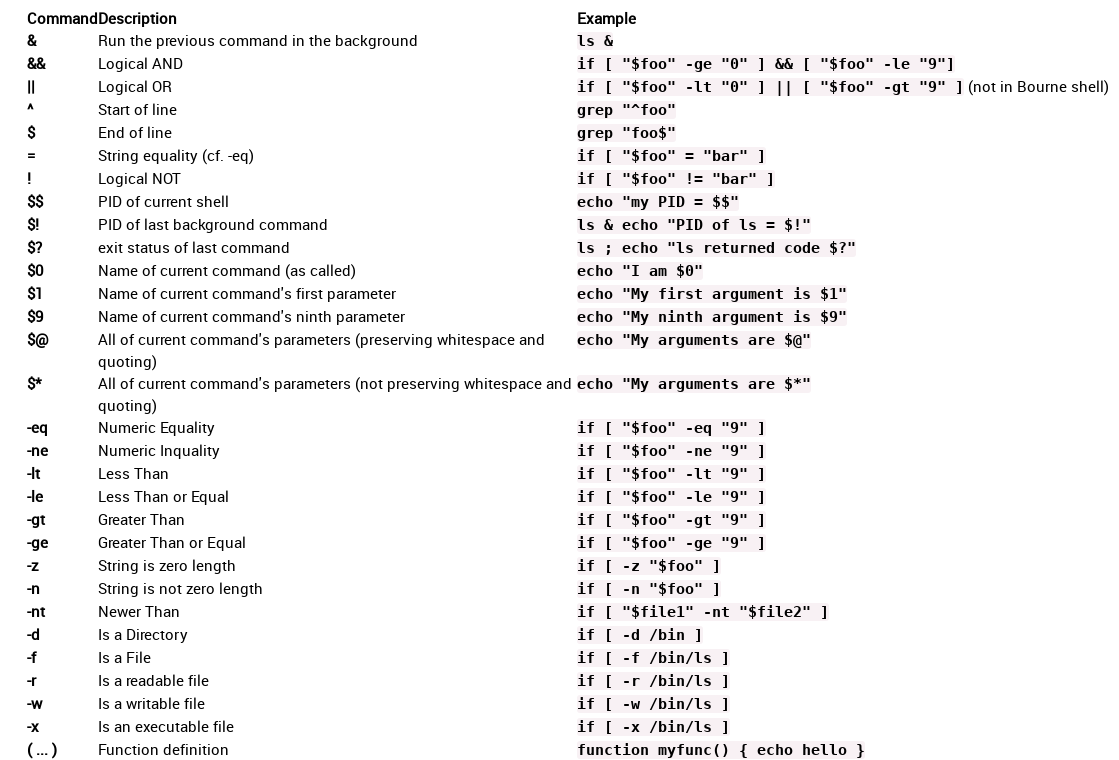
\includegraphics[height=12cm]{referencias.png}
\end{center}

\subsection*{Shell Interactivo}

Shell tambien puede ser usado mediante otras formas que no son scripts. Primeramente bash tiene algunas herramientas de búsqueda de historia muy prácticas; las teclas de flecha hacia arriba y hacia abajo se desplazarán por el historial de comandos anteriores. Más útilmente, Ctrl + r hará una búsqueda inversa, haciendo coincidir cualquier parte de la línea de comando. Presione ESC y el comando seleccionado se pegará en el shell actual para que pueda editarlo según sea necesario. Por otra parte el ksh se le pueden agregar comandos del historial, es posble abrir una nueva sesión ksh desde otro shell interactivo, y luego regresar al anterior.

\section*{Conclusión}
En general el realizar tanto la práctica como el presente reporte fue ineteresante, ya que se enlazó bastante la teoría con lo práctico, además de que es la primera vez que se trabaja con shell script. Algo que en lo personal era desconocido en un principio para mi, por que se habia estado trabajando con lenguajes interpretados. Sin pensar ya estabamos haciendo scripts. Con bastante esfuezo y sobre todo análisis e interpretación de teoría se llegó a concluir con la actividad.

\section*{Bibiografía}
\begin{itemize}
\item Atmospheric Soundings. (2018). Weather.uwyo.edu. Recuperado el 16 de Febrero de 2018, desde http://weather.uwyo.edu/upperair/sounding.html
\item  Comandos de Linux mas frecuentemente utilizados. (2018). Linuxtotal.com.mx. \\Recuperado el 20 de Febrero de 2018, desde \\https://www.linuxtotal.com.mx/?cont=info\_admon\_002
\item  Shell de Unix. (2018). Es.wikipedia.org. Recuperado el 19 de Febrero de 2018, desde https://es.wikipedia.org/wiki/Shell\_de\_Unix
\item  Shell Scripting Tutorial. (2018). Shellscript.sh. Recuperado el 21 de Febrero de 2018, desde https://www.shellscript.sh/index.html
\end{itemize}
\newpage
\section*{Apéndice}
\begin{enumerate}
\item ¿Qué fue lo que más te llamó la atención en esta actividad?\\
\textit{Primeramente el uso de nuevos comandos con el interprete de comandos de Unix, recuerdo que en el curso de Programación y Lenguaje Fortran en las prácticas introductorias hablamos sobre algunos de ellos que generalmente eran para la creación de directorios, los vistos aquí se podria decir que son de mas nivel. Claro, destacando tambien que el uso de scripts es una herramienta muy util para automatizar el uso de comandos que fueron presentados.}
\item ¿Qué consideras que aprendiste?\\
\textit{En general, el uso de scripts como una forma de automatizar y también de forma manual.}
\item ¿Cuáles fueron las cosas que más se te dificultaron?\\
\textit{La manera de utilizar los comandos, ya que cambian de una forma a otra y es diferente como se trabajan.}
\item ¿Cómo se podría mejorar en esta actividad? \\
\textit{Pienso que es necesario prácticar con los comandos y tener una explicación teórica (origen, uso y manera de abreviación) de ellos, en las que se propongan ejercicios interactivos para su comprensión.}
\item ¿En general, cómo te sentiste al realizar en esta actividad?\\
\textit{Tenía inseguridad en un principio, pues me di cuenta que sería complicado por que me iba a enfrentar a algo nuevo, por el lado de la síntesis, la información de ella estaba en inglés y se me iba a complicar por mi nivel de comprensión, pero conforme el desarrollo, aunque estuvo bastante larga logré terminarla.}
\end{enumerate}





\section*{}

\end{document}
